\chapter{多无人机SLAM仿真} \label{Simulation}

% 介绍框架
本章主要多无人机SLAM的仿真;为了循序渐进,首先介绍仿真环境的配置,其次是单机的SLAM仿真,最后过渡到多机的SLAM仿真。


\section{gazebo仿真环境配置}

在进行仿真之前,首先要对场景进行搭建,对launch文件进行配置。

\subsection{场景} \label{4.1.1}

仿真环境中,场景的设计不能过于简单,墙壁、地面等大面积重复物体应该具有纹理,否则ORB-SLAM2的特征点提取会十分困难;除了纹理的设计,还应尽可能多地提供物体,使场景丰富。如图\ref{fig3-1}所示:

\begin{figure}[!ht]
	\centering
	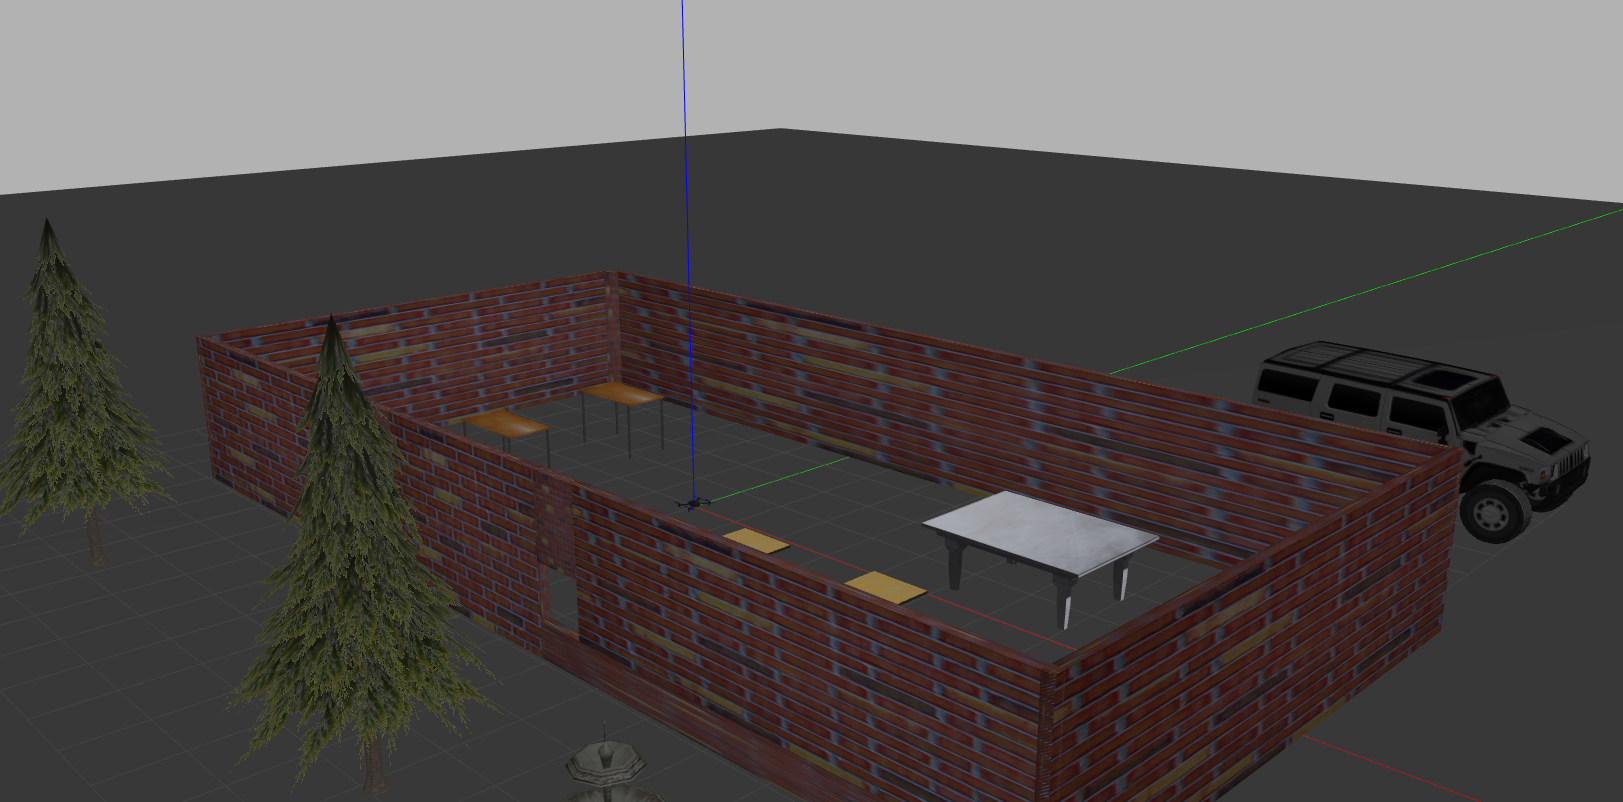
\includegraphics[width=0.7\textwidth]{scene.png}
	\caption{gazebo场景示例}
	\label{fig3-1}
\end{figure}

进入gazebo界面后,使用Control+B进入其编辑界面;之后有两种选择:

\begin{enumerate}
	\item 建立基础模型,一般在这里会绘制上地面及其纹理;如果是室内场景,还会绘制一个大致的墙壁结构,墙壁的纹理,其上的门窗等;最后将该模型保存到.gazebo/model文件中,这是gazebo模型的默认文件。
	\item 直接选择插入模型;可以在此直接插入上文建立的基础模型,也可以插入其他模型库已有的模型,默认存储在/.gazebo/models文件夹下
\end{enumerate}

最后需要将自建场景存储为一个.world文件,gazebo不会给文件后缀的提示,需要自己输入后缀,这一点需要特别注意。在此之后,就获得了自建的world场景,下一步需要在launch文件中更改该项,完成调用。


\subsection{launch文件} \label{4.1.2}

\ref{2.1.2}节中,曾简单介绍launch文件的功能。作为整个仿真环境的配置文件,launch文件中基本包含了仿真所需的参数。

launch文件使用XML标签语言书写,主要为确定启动的节点和加载参数使用,简单的开始节点、加载参数的方法如下:

\begin{lstlisting}[language={XML}]
<node pkg="your package name" name="your node name" type="your node type"/>
<param name="param name" value="param value"/>
<arg name="arg name" default="arg value"/>
\end{lstlisting}

在一个简单的launch文件中,主要会包括设备的信息设置、PX4配置和gazebo仿真配置。

\begin{enumerate}
	\item 
\end{enumerate}




\section{单机SLAM仿真}
\subsection{EKF设置及启动仿真} \label{4.2.1}
\subsection{视觉定位的坐标变换} \label{4.2.2}

\section{多机SLAM仿真}
